%Slide template for use by PCFC / HGD / SWL, etc. (Prof. K. Alexander Heufer)
%Developed by Mark E. Fuller from examples and miscellany produced at RWTH Aachen
%(probably mostly from the work of Philippe Dreuw and Thomas Deselaers)
%This template copyright Mark E. Fuller, 2021 (mark.e.fuller@gmx.de)

\documentclass[10pt,presentation]{beamer}

%%%%%%%%%%%%%%%%%%%%%%%%%%%%%%%%%%%%%
%% Select input file encoding:
%%   utf8   - UTF-8, nowadays standard on most operating systems
%%   latin1 - ISO-8859-1
\usepackage[utf8]{inputenc}

%%%%%%%%%%%%%%%%%%%%%%%%%%%%%%%%%%%%%
%% Select language
%%
\usepackage[ngerman]{babel}        % Deutsch, neue Rechtschreibung
%\usepackage[english]{babel}       % English

\usetheme{rwth}
\usepackage[T1]{fontenc}           % Font encoding (don't change!)
\usepackage{lmodern}               % Select Linux Modern Fonts (don't change)
\usepackage{sansmathfonts}         % Sans fonts in math environments
\usepackage{textcomp}              % fix 'missing font symbols' warning
\renewcommand{\rmdefault}{phv}     % Arial like (Helvetica)
\renewcommand{\sfdefault}{phv}     % Arial like (Helvetica)

%% graphics related packages
\usepackage{graphicx}              % needed to include graphics (don't change)
\usepackage{epstopdf}              % required to include eps files
%\usepackage{svg}                   % include svg files (requires Inkscape)
\usepackage[encoding,filenameencoding=utf8]{grffile} % allow utf8 file names in graphics

%%%%%%%%%%%%%%%%%%%%%%%%%%%%%%%%%%%%%
%% import packages for content
%%
\usepackage{listings}                           % for lstlisting and \lstinline|..|
%% TikZ can be used to /program/ graphics.
\usepackage{tikz}                                % comment-out, if you don't need this.
%% some TikZ-libraries and settings for the examples...
\usetikzlibrary{shadings}           % GW: color gradients
\usetikzlibrary{arrows,calc,positioning,fit,matrix,shadows,chains,arrows,shapes,spy,fadings}
\usepackage{pgfplots}
\usetikzlibrary{pgfplots.units,shapes.symbols,shapes.arrows}
%\usetikzlibrary{pgfplots.external}
%\tikzexternalize[prefix=tmp/]

%% Custom packages and definitions

% Mathematikumgebung
\usepackage{amsmath}
\usepackage{amssymb}
\usepackage{sansmath}

% tabularx -> bessere "tabular"-Umgebung
\usepackage{tabularx}

% zusätzliche Formatbezeichner für die tabularx-Umgebung
\newcolumntype{L}{>{\raggedright\let\newline\\\arraybackslash\hspace{0pt}}X}
\newcolumntype{R}{>{\raggedleft\let\newline\\\arraybackslash\hspace{0pt}}X}
\newcolumntype{C}{>{\centering\let\newline\\\arraybackslash\hspace{0pt}}X}

% center text vertically in tabularx(column)
%\renewcommand{\tabularxcolumn}[1]{>{\large}m{#1}}

% Bessere Tabellenlinien
\usepackage{booktabs}

% Tabellenzeilen für booktabs anpassen -> call on frame with table
\newcommand{\fixbooktabsrowhight}{%
    \setlength{\aboverulesep}{0pt}
    \setlength{\belowrulesep}{0pt}
    \setlength{\extrarowheight}{.5ex}
}

% Zellen über mehrere Zeilen
\usepackage{multirow}

% Source, e.g. for images
\setbeamercolor{framesource}{fg=gray}
\setbeamerfont{framesource}{size=\tiny}

\usepackage[absolute,overlay]{textpos}
\newcommand{\source}[1]{\begin{textblock*}{\linewidth}(1ex,\paperheight-2.75em)
        \begin{beamercolorbox}[left]{framesource}
            \usebeamerfont{framesource}\usebeamercolor[fg]{framesource} Source: {#1}
        \end{beamercolorbox}
\end{textblock*}}

\usepackage{etoolbox}
%% short titles for toc \(sub)section[SHORTTITLE for toc]{LONGTITLE for slide}
\makeatletter
% Insert [short title] for \section in ToC
\patchcmd{\beamer@section}{{#2}{\the\c@page}}{{#1}{\the\c@page}}{}{}
% Insert [short title] for \section in Navigation
\patchcmd{\beamer@section}{{\the\c@section}{\secname}}{{\the\c@section}{#1}}{}{}
% Insert [short title] for \subsection in ToC
\patchcmd{\beamer@subsection}{{#2}{\the\c@page}}{{#1}{\the\c@page}}{}{}
% Insert [short title] for \subsection  in Navigation
\patchcmd{\beamer@subsection}{{\the\c@subsection}{#2}}{{\the\c@subsection}{#1}}{}{}
\makeatother

%% MEF packages and commands
\usepackage{multicol}
\usepackage[version=3]{mhchem} % Formula subscripts using \ce{}
\newcommand{\nox}{NO$_x$} % our abbreviation
\usepackage{subfigure}
\usepackage{scrextend} %needed for footnotes in tables
\DeclareRobustCommand{\ILS}{
\includegraphics[height=\fontcharht\font`T]{/home/fuller/Dropbox/Documents/TeX/ILS_bold}}

%get proper bib with numbered entries
%\setbeamertemplate{bibliography item}{\insertbiblabel}

%footnote citations - replace \cite with \footcite or \footfullcite
\usepackage[backend=bibtex, style=chem-acs]{biblatex} %, style=authoryear-comp
\addbibresource{../sample.bib}

%shrink citations
\setbeamerfont{footnote}{size=\tiny}

%no ``figure'' in caption
\setbeamertemplate{caption}{\insertcaption} 

\newcommand{\red}[1]{\textcolor{red}{#1}} %easy red text
\usepackage{ulem}
\newcommand{\soutthick}[1]{%
	\renewcommand{\ULthickness}{1.6pt}%
	\sout{#1}%
	\renewcommand{\ULthickness}{.4pt}% Resetting to ulem default
}

%add YAML to listings: https://www.latex4technics.com/?note=187E
\newcommand\YAMLcolonstyle{\color{red}\mdseries}
\newcommand\YAMLkeystyle{\color{black}\bfseries}
\newcommand\YAMLvaluestyle{\color{blue}\mdseries}

\makeatletter

% here is a macro expanding to the name of the language
% (handy if you decide to change it further down the road)
\newcommand\language@yaml{yaml}

\expandafter\expandafter\expandafter\lstdefinelanguage
\expandafter{\language@yaml}
{
	keywords={true,false,null,y,n},
	keywordstyle=\color{darkgray}\bfseries,
	basicstyle=\YAMLkeystyle,                                 % assuming a key comes first
	sensitive=false,
	comment=[l]{\#},
	morecomment=[s]{/*}{*/},
	commentstyle=\color{purple}\ttfamily,
	stringstyle=\YAMLvaluestyle\ttfamily,
	moredelim=[l][\color{orange}]{\&},
	moredelim=[l][\color{magenta}]{*},
	moredelim=**[il][\YAMLcolonstyle{:}\YAMLvaluestyle]{:},   % switch to value style at :
	morestring=[b]',
	morestring=[b]",
	literate =    {---}{{\ProcessThreeDashes}}3
	{>}{{\textcolor{red}\textgreater}}1     
	{|}{{\textcolor{red}\textbar}}1 
	{\ -\ }{{\mdseries\ -\ }}3,
}

% switch to key style at EOL
\lst@AddToHook{EveryLine}{\ifx\lst@language\language@yaml\YAMLkeystyle\fi}
\makeatother

\newcommand\ProcessThreeDashes{\llap{\color{cyan}\mdseries-{-}-}}

\title{Progress in \soutthick{ Nitrogen } Novel Combustion Chemistry}
%\subtitle{Subtitle}
%\titlegraphic{}
\author{Mark E. Fuller, Ph.D.}
\email{fuller@pcfc.rwth-aachen.de} % optionally
\institute{Physico-Chemical Fundamentals of Combustion}
%\webaddress{www.informatik.rwth-aachen.de/mentoring} % overrides www.rwth-aachen.de
\date{\today}
\subject{RWTH presentation template}
\keywords{RWTH, Latex Beamer, template}

%\logo{\includegraphics[height=8mm]{logos/logo}} % will replace the default logo

% official institute logo offset correction
%\logo{\vskip-3.5mm\includegraphics[height=12.5mm]{logos/rwth_mentoring_rgb.eps}\hspace{-2mm}} % optionally
\logo{\vskip-2mm
\includegraphics[width=45mm]{../figures/Logos/RWTH/PCFC.png}\hspace{-2mm}} % optionally

% alternative logo position (not recommended)
%\instlogo{\includegraphics[height=10mm]{logos/rwth_mentoring_rgb.eps}} % optionally

%%%%%%%%%%%%%%%%%%%%%%%%%%%%%%%%%%%%%
%% configure template behaviour
%%-------------------------------
%%   secstart -- style of section start
%%               selectable parameters:
%%                 sectitle:  only provides section title
%%                 sectoc:    display section table of contents
%%                 <empty>:   display nothing on section start
\secstart{sectitle}
% disable PDF navigation icons
\setbeamertemplate{navigation symbols}{}

\begin{document}
    
\begin{frame}{\nox\ interactions in hydrocarbon combustion}
    \begin{figure}
        \centering
        \includegraphics[width=0.8\linewidth]{../figures/NOx_Cycle.png}
        \caption{And when \ce{RH} is replaced with \ce{QOOH} or \ce{OOQOOH}?}
        \label{fig:NOx_cycle}
    \end{figure}
\end{frame}


\begin{frame}{Latest revisions}
    \begin{itemize}
        \item The \ce{HNO2} potential energy surface (PES) reactions calculated by Chen {\it et al.}\footfullcite{Chen.2019}
        \item Rates for the \ce{H2NO2} and \ce{CH4NO2} PES from Fuller and Goldsmith\footfullcite{Fuller.2018}
        \item Hydrogen abstraction by \ce{NO2} from alkanes and alkenes refit to the exothermic direction\footfullcite{Fuller.2018, Fuller.2020}
        \item Decomposition rates for alkyl nitrites\footfullcite{Randazzo.2018}, and isopropyl nitrate\footfullcite{Fuller.2019.A}
    \end{itemize}
\end{frame}

\begin{frame}{Reaction Classes and Examples}
    Develop mechanism by systematic inclusion of reaction classes
    \begin{itemize}
        \item Hydrogen abstractions by \nox to form \ce{HONO}, \ce{HNO2}, \ce{HNO}
        \item Unimolecular conformer formation and dissociation
        \begin{itemize}
            \item \ce{RNO2}$\rightleftharpoons$ \ce{R} + \ce{NO2}
            \item \ce{RONO}$\rightleftharpoons$ \ce{RO} + \ce{NO}
            \item \ce{RONO2}$\rightleftharpoons$ \ce{RO} + \ce{NO2}
        \end{itemize}
        \item Isomerizations  
        \begin{itemize}
            \item \ce{RONO}$\rightleftharpoons$ \ce{RNO2}
        \end{itemize}
        \item Concerted \ce{HONO} elimination
        \begin{itemize}
            \item \ce{RONO}$\rightleftharpoons$ alkene + \ce{HONO}
        \end{itemize}
        \item \nox\ cycling reactions
        \begin{itemize}
            \item \ce{RO2} + \ce{NO} $\rightleftharpoons$ \ce{RO} + \ce{NO2}
            \item \ce{RO} + \ce{NO} $\rightleftharpoons$ \ce{R} + \ce{NO2}
        \end{itemize}
    \end{itemize}
\end{frame}

\begin{frame}{The old (slow) way forward}
	\begin{multicols}{2}
	\begin{enumerate}
		\item Calculate sensitivities
		\item Tweak/add some rates*
		\item Run simulations
		\item Feel sad and start over
	\end{enumerate}
	\columnbreak
	\centering
	{\scriptsize *Until this...\\}
	\vspace{0.1cm}
	\includegraphics[width=0.8\columnwidth]{../figures/NOx_Cycle.png}
	\vspace{0.1cm}
	{\scriptsize ...becomes this (or worse!)}
	\vspace{0.1cm}
	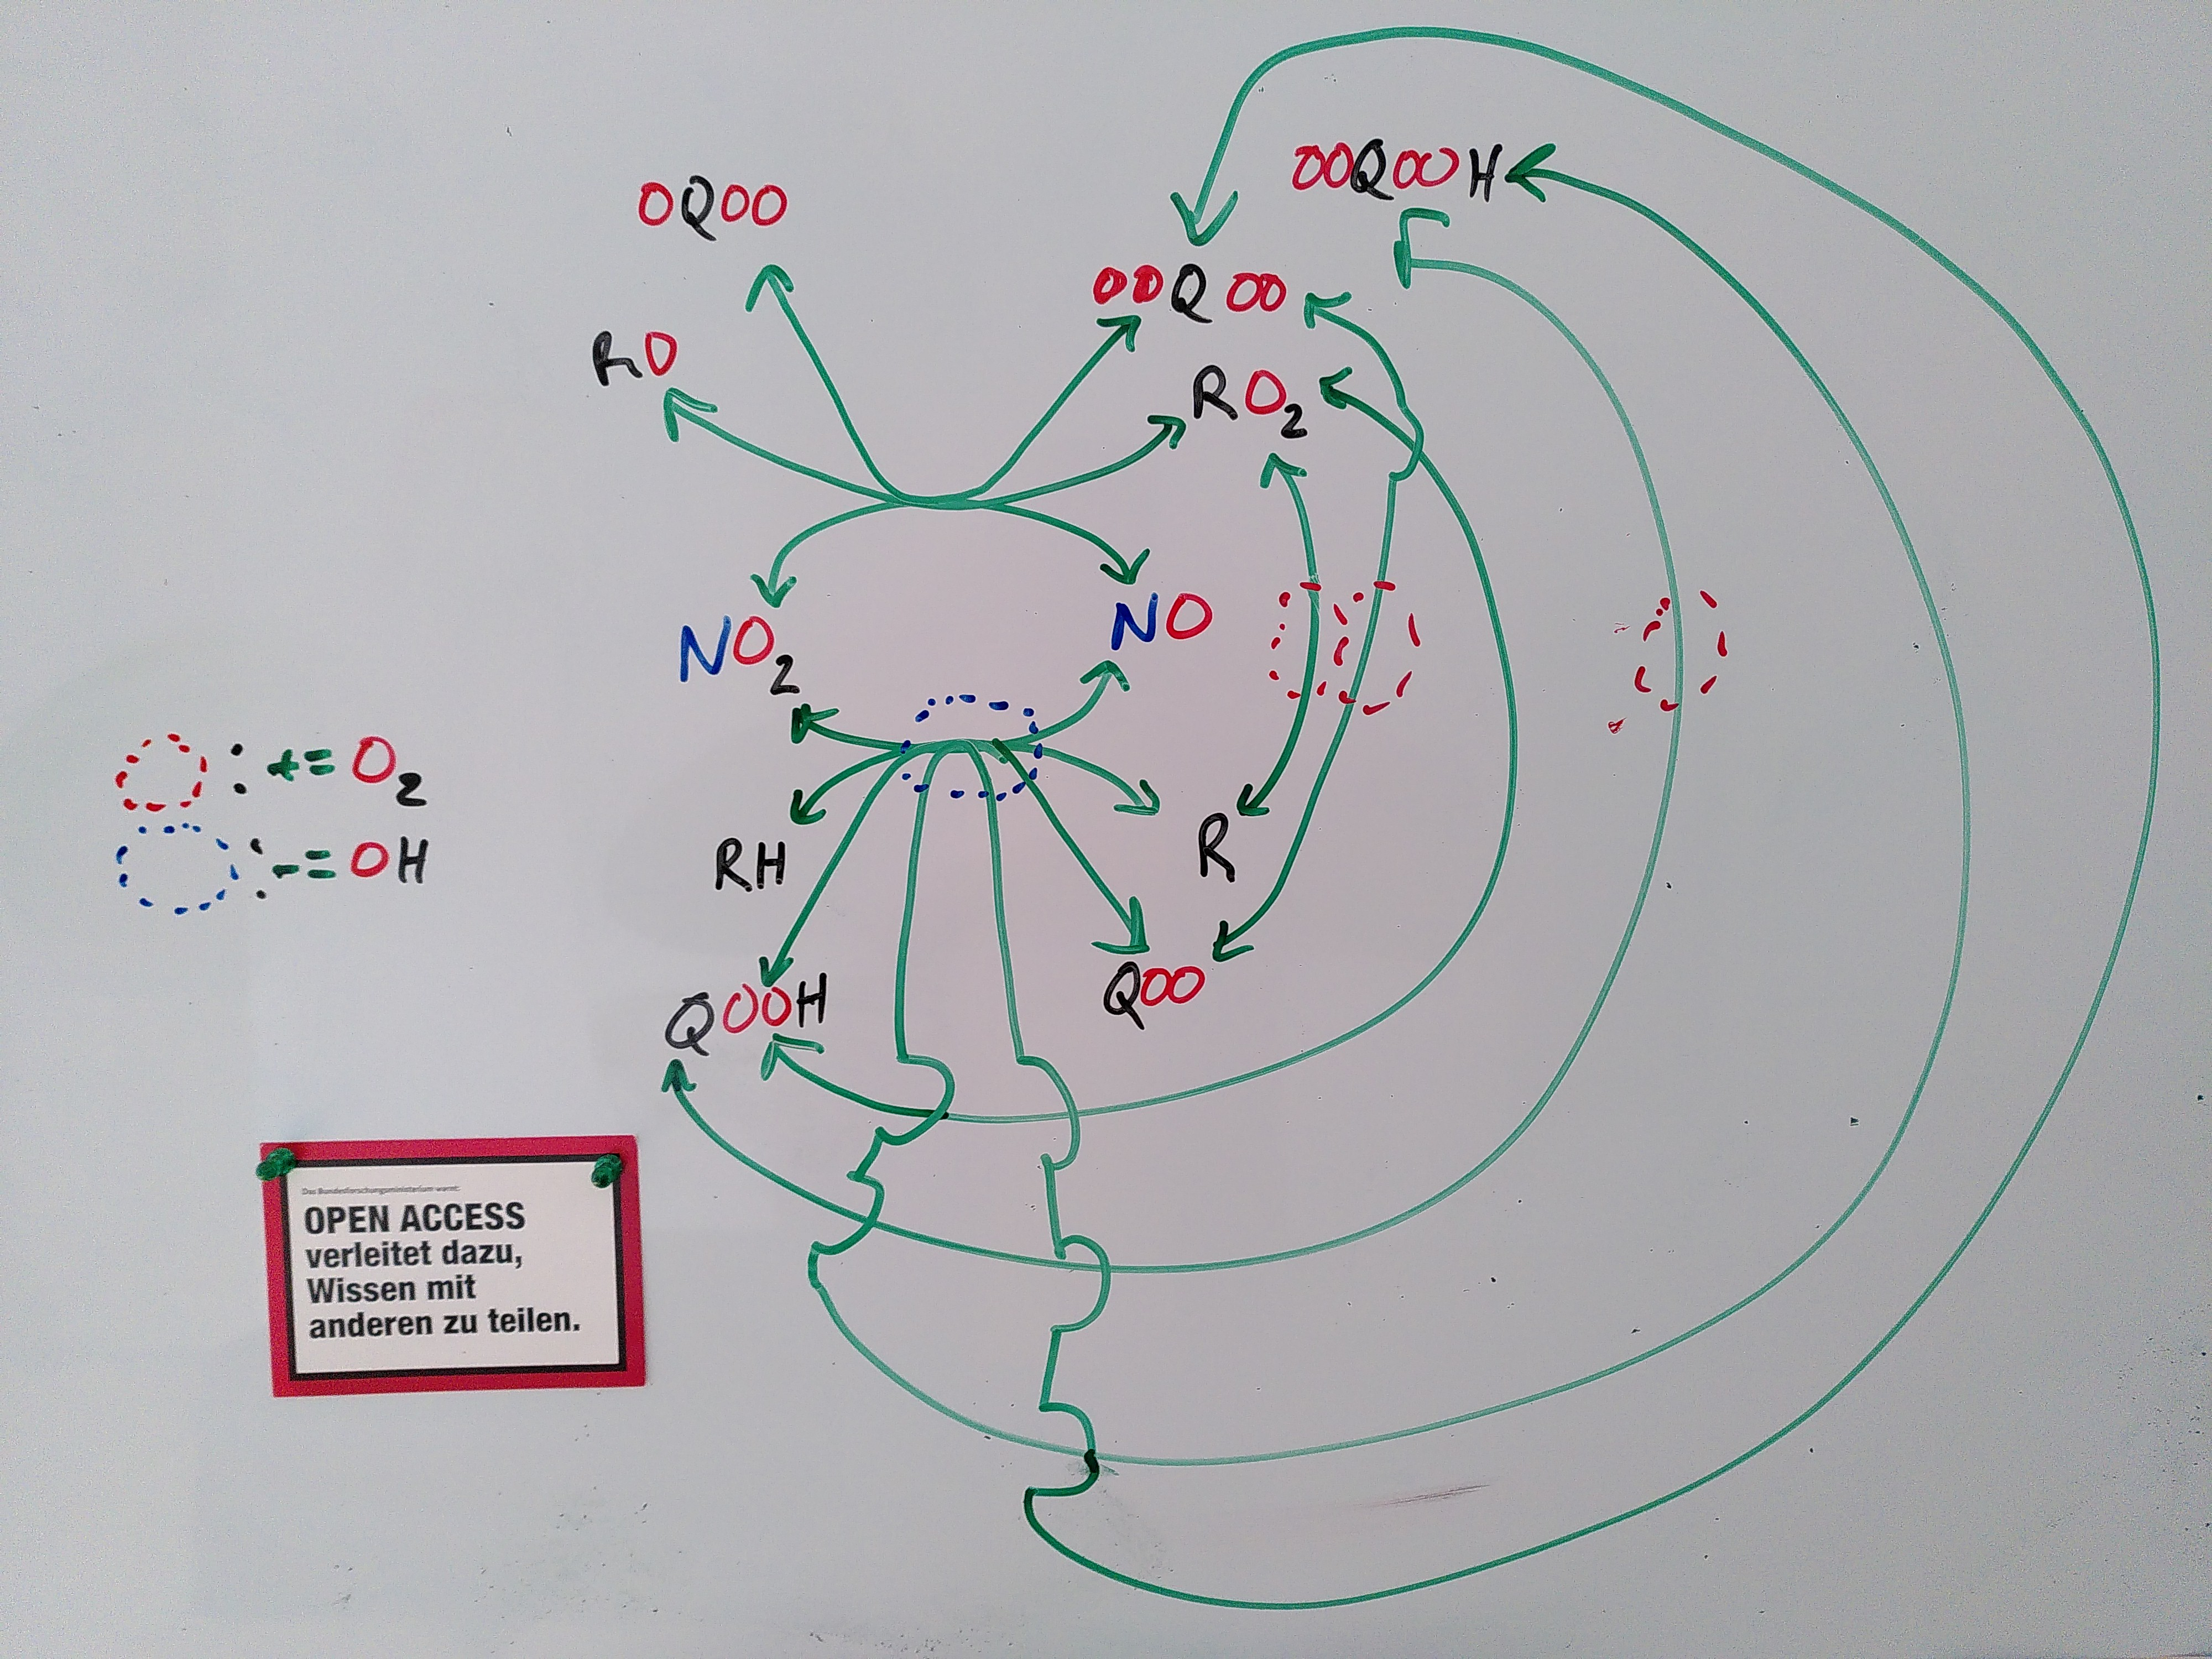
\includegraphics[width=0.8\columnwidth]{../figures/BigNOxCycle.jpg}
	\end{multicols}
\end{frame}

\begin{frame}{Progress on \nox-Cycling}
	\begin{figure}
		\centering
		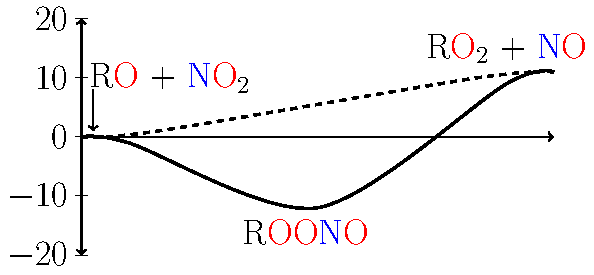
\includegraphics[width=0.5\columnwidth]{../figures/PES_NOx-Cycle.pdf}
		\caption{Generalized potential energy surface for alkoxy radical (RO) + \ce{NO2} system. Energies in kcal/mol.
			Well-skipping occurs at virtually all combustion-relevant temperatures and pressures.}
		\label{fig:NOx-Cycle_PES}
	\end{figure}
\begin{tabular}{crrr}
	\toprule
	Reaction & \multicolumn{1}{c}{$A$} & \multicolumn{1}{c}{$n$} & \multicolumn{1}{c}{$E_a$}\\
	\midrule
	\ce{CH3O2} + \ce{NO} $\rightleftharpoons$ \ce{CH3O} + \ce{NO2} & 4.62E+15 & -0.38 & 97.8\\
	\ce{C2H5O2} + \ce{NO} $\rightleftharpoons$ \ce{C2H5O} + \ce{NO2} & 2.11E+14 & -0.12 & -470.6\\
	\ce{NC3H7O2} + \ce{NO} $\rightleftharpoons$ \ce{NC3H7O} + \ce{NO2} & 1.07E+14 & -0.25 & -1302.0\\
	\bottomrule
\end{tabular}	

Units: centimeters, kelvin, calories, moles
\end{frame}

%\printbibliography

\end{document}